\label{chapter:conformingsubdivision}

The following chapters result are due to Hersherberger and Suri\cite{HershbergerS99}. 
We will present the main theory behind a conforming subdivision, 
and an algorithm for computing it, and The impleman 

Given a plane with obstacles, we could view this as a plane with holes in it, which we 
cannot enter. These holes are made of the obstacles occupying the space. So here the notion 
of free space is the plane minus the interior of the obstacles. This free space is where the 
unmodified Hershberger-Suri would find a shortest path, that is a shortest path without 
violations. One of the key ideas for calculating the shortest path map, which we need to 
find the shortest path, is the notion of a conforming subdivision of the free space. This is 
a subdivision of the free space into squares, which we will call \textit{cells}, where a 
cell has a constant descriptives complexity. 

This construction is done i two steps: the 
first step construct a subdivision while only considering the vertices of the obstacle 
polygons. The second step will then insert the obstacle edges into the subdivision, which 
will have a taken a grid-like structure. This structure is build bottom up, such that every 
vertex in the plane is contained in the interior of a cell. The algorithm then proceeds to 
simulate \textit{growth-process} which will make the cells grow until then entire plane is 
covered by these cells. The way this growth is facilitated is by defining a equivalence 
class of when cells overlap, and can be merged together. This is the reason it's called a 
conforming subdivision, since the grid grows, and conforms to the vertices in the plane. 


When this grid of orthogonal cells has been produced we insert the obstacle edges intro the 
grid, giving us two types of edges. The edges that we have grown, which we will call 
\textit{transparent} edges, since our wavefronts will be able to pass through them, and the 
obstacles edges which we will call \textit{opaque} edges, which the wavefront will be 
blocked by these. The transparent edges will obey the claim that the will be well-covered, 
which we will define in the next section, but this help us bind the overall complexity of 
the subdivision, and secure that there are $O(1)$ of cells within a distance of $2|e|$ for 
every transparent edge $e$. It is this well-covering property that the shortest path 
algorithm relies heavy on, in the unmodified Hershberger-Suri algorithm. This subdivision 
can be built in $O(n \log n)$ time \cite{HershbergerS99}.

\section{Defining well covering of regions}\label{section:def-well-covering-if-regions}

A crucial property of the quad-like subdivision is the subdivision being \textit{well-
covering} on its internal edges. The following section outlines the different definitions 
and properties that we mean by well-covering, This section is very much inspired by 
Hershberger and Suri definition for the same concepts in \cite{HershbergerS99}. 

We give the following definition for well-covering:

\begin{mydef}
	\label{def:wellcoveringwithpara}
	\textbf{Well-covering with parameter $\alpha$:}\\
	Given a straight line subdivision $\mathcal{S}$ of the plane, an edge
	$e\in\mathcal{S}$ is said to be \textit{well-covered with parameter}
	$\alpha$ if the following three conditions hold:
	\begin{enumerate}
    \setlength\itemsep{1em}
		\item[W1.] There exists a set of cells $\mathcal{C}(e)\subseteq\mathcal{S}$ such
				   that $e$ lies in the interior of their union. The union is denoted
				   $\mathcal{U}(e)=\{c|c\in\mathcal{C}(e)\}$.
		\item[W2.] The total complexity of all the cells in $\mathcal{C}(e)$ is 
        		   $O(\alpha)$.
		\item[W3.] If $f$ is an edge on the boundary of the union $\mathcal{U}(e)$, then
        		   the Euclidean distance between $e$ and $f$ us at least $\alpha\cdot
				   max(|e|,|f|)$. 
	\end{enumerate}
	The edge is said to be \textit{strongly} well-covered if the stronger
	condition 3' holds:
	\begin{enumerate}
    \setlength\itemsep{1em}
		\item[W3'.] If $f$ is an edge on \textit{or outside} the boundary of the
					union $\mathcal{U}(e)$, then the Euclidean distance between $e$ and
					$f$ is at least $\alpha\cdot max(|e|,|f|)$.
	\end{enumerate}
\end{mydef}

In either of the two cases, we will say the region $\mathcal{U}(e)$ is called
the \textit{well-covering region of e}. The Hershberger-Suri shortest path algorithm 
focuses solely on the distance from the boundary of $\mathcal{U}(e)$ to $e$, which means 
we only require a the region to be well-covered, and not strongly well-covered. The 
reason for a definition of strongly well-coveredness is due to the definition being 
used later for proving correctness of algorithm.

\begin{mydef}
	\label{def:aconformingsubdivision}
	\textbf{$\alpha$-conforming subdivision:} \\
	Let $V$ denote the set of vertices of the obstacle polygons, plus the source
	vertex $s$. A subdivision $\mathcal{S}$ is called a \textit{(strong)
	$\alpha$-conforming subdivision for V} if:
	\begin{enumerate}
    \setlength\itemsep{1em}
		\item[C1.] Each cell of $\mathcal{S}$ contains at most one point of $V$ in its
				   closure\footnote{its interior plus boundary}.
		\item[C2.] Each edge of $\mathcal{S}$ is (strongly) well-covered with
				   parameter $alpha$.
		\item[C3.] The well-covering region of every edge of $\mathcal{S}$ contains at
				   most one vertex of $V$.
	\end{enumerate}
\end{mydef}

The reason for the naming of definition \ref{def:aconformingsubdivision} being 
conforming, is due to condition 1 and 3, will force the cell structure to 
\textit{conform} around the distribution of the point of $V$, and example of can be seen 
in Figure \ref{fig:1conformingsubdivision}. Since the Hershberger-Suri
constructs a 2-conforming subdivision $V$, we will the rest of the thesis
denote \textit{conforming} to 
mean 2-conforming, and explicitly state the parameter if it is 
not 2. 

\begin{figure}
	\centering
	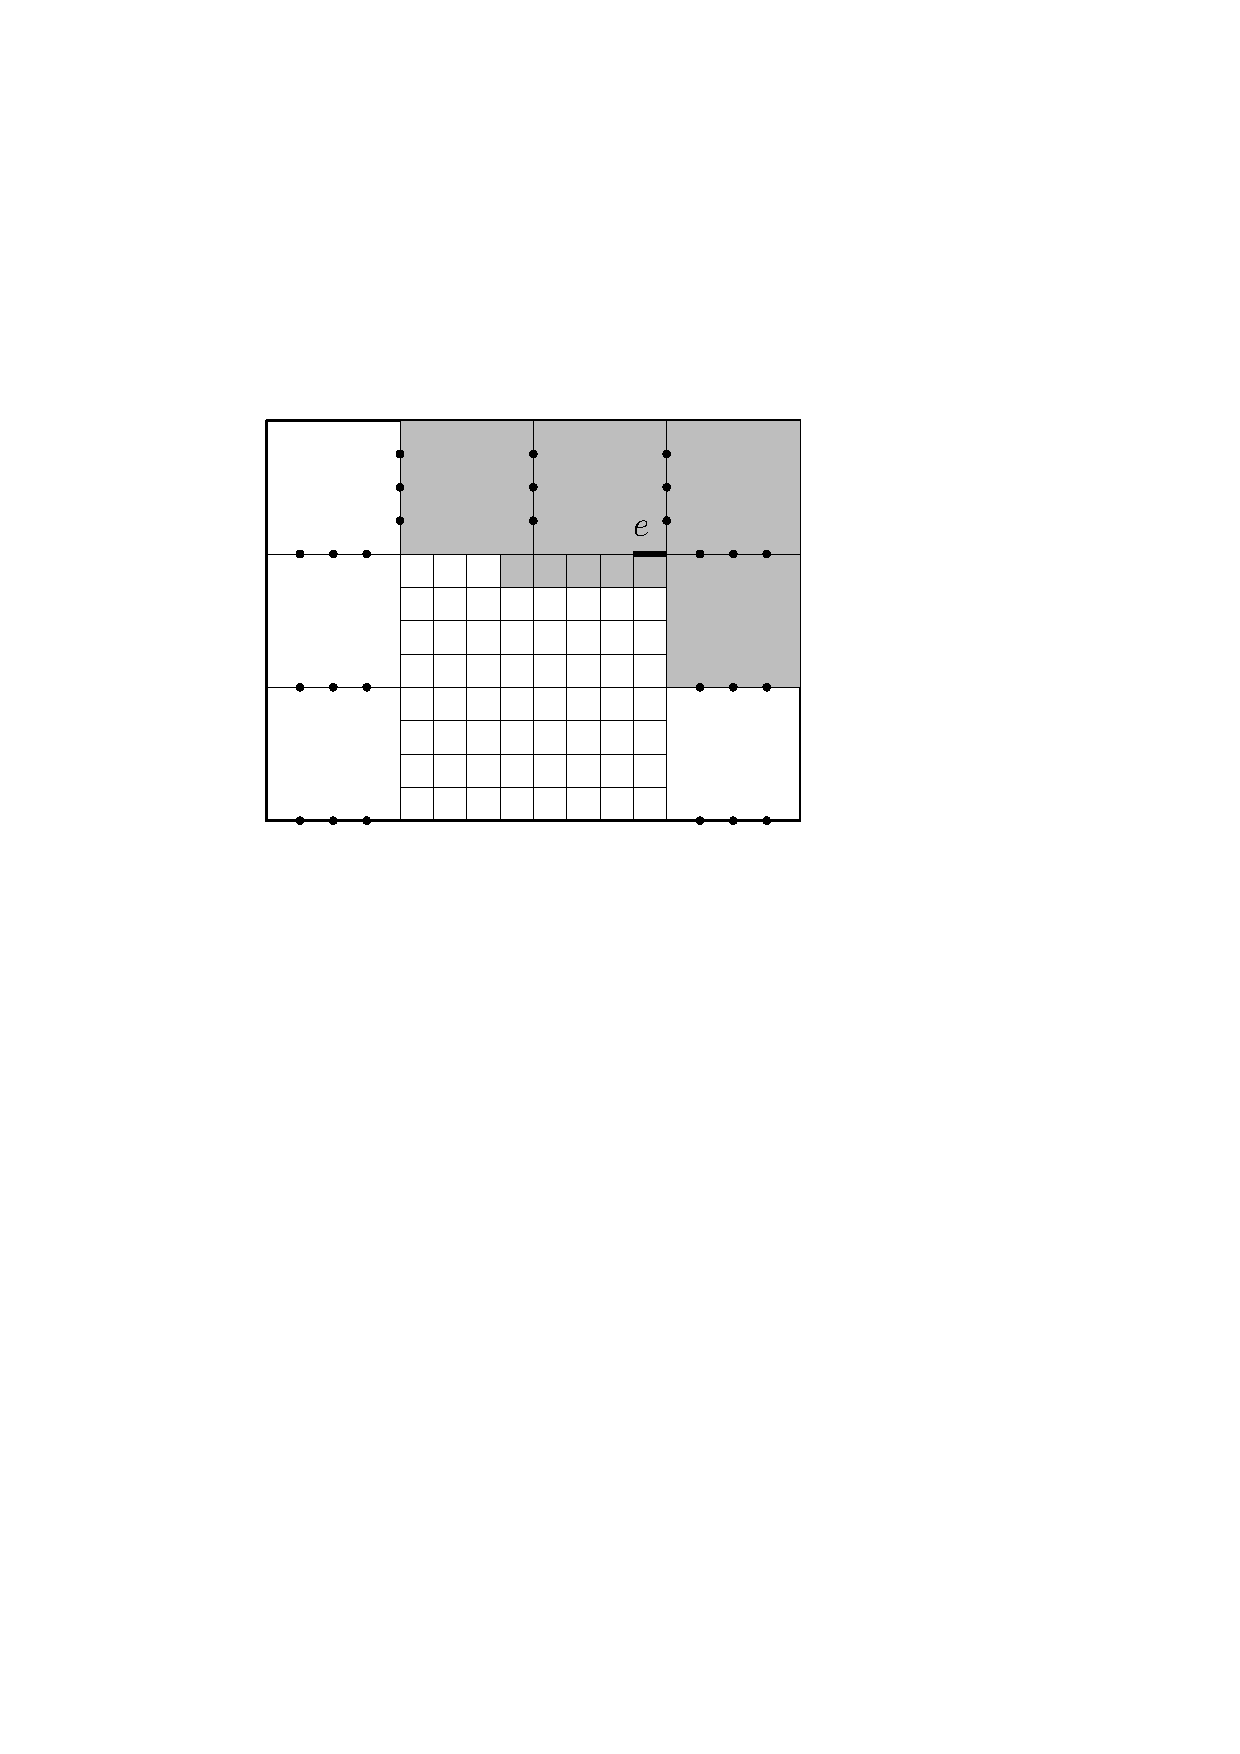
\includegraphics[width=0.5\textwidth]{figures/1conformingsubdivision.pdf}
	\caption{An example of part of an string 1-conforming subdivision. The shaded region 
    		 in the figure is the union of cell $\mathcal{U}(e)$ forming a well-covering 
             of edge $e$}
	\label{fig:1conformingsubdivision}
\end{figure}

As mentioned earlier in the overview of the Hershberger-Suri algorithm, the subdivision of 
$\mathcal{S}$ is similar to a quad-tree in that all its edges are horizontal or vertical. 
However, as we will see, the cells of $\mathcal{S}$ may not always be convex and the 
subdivision itself can be disconnected. As will shown later, each cell is still reasonably 
well-behaved, and there are at most one hole per cell. To give a more precise definition, 
each cell is either a square or a square-annulus.

\begin{mydef}
	\textbf{(Square-annulus:)}\\
	We will define it as a square $A$ which is missing  a square $B$ internally such that 
    the internal square $B$ is at least $1/4$ the side length of the outer square $B$
\end{mydef}

But the boundary of these cell may be subdivide into a constant number of edges.
We require also that they have the following minimum clearance property: 

\begin{mydef}
\textbf{(Minimum clearance property:)} \label{minimumclearanceproperty}\\
      The minimum width of an annulus in the subdivision (the minimum distance from the 
      inner square to the outer square) is at least one quarter of the side length of the 
      outer square. See Figure \ref{fig:minimumclearancesquareannulus}
\end{mydef}

\begin{figure}[H]
	\centering
	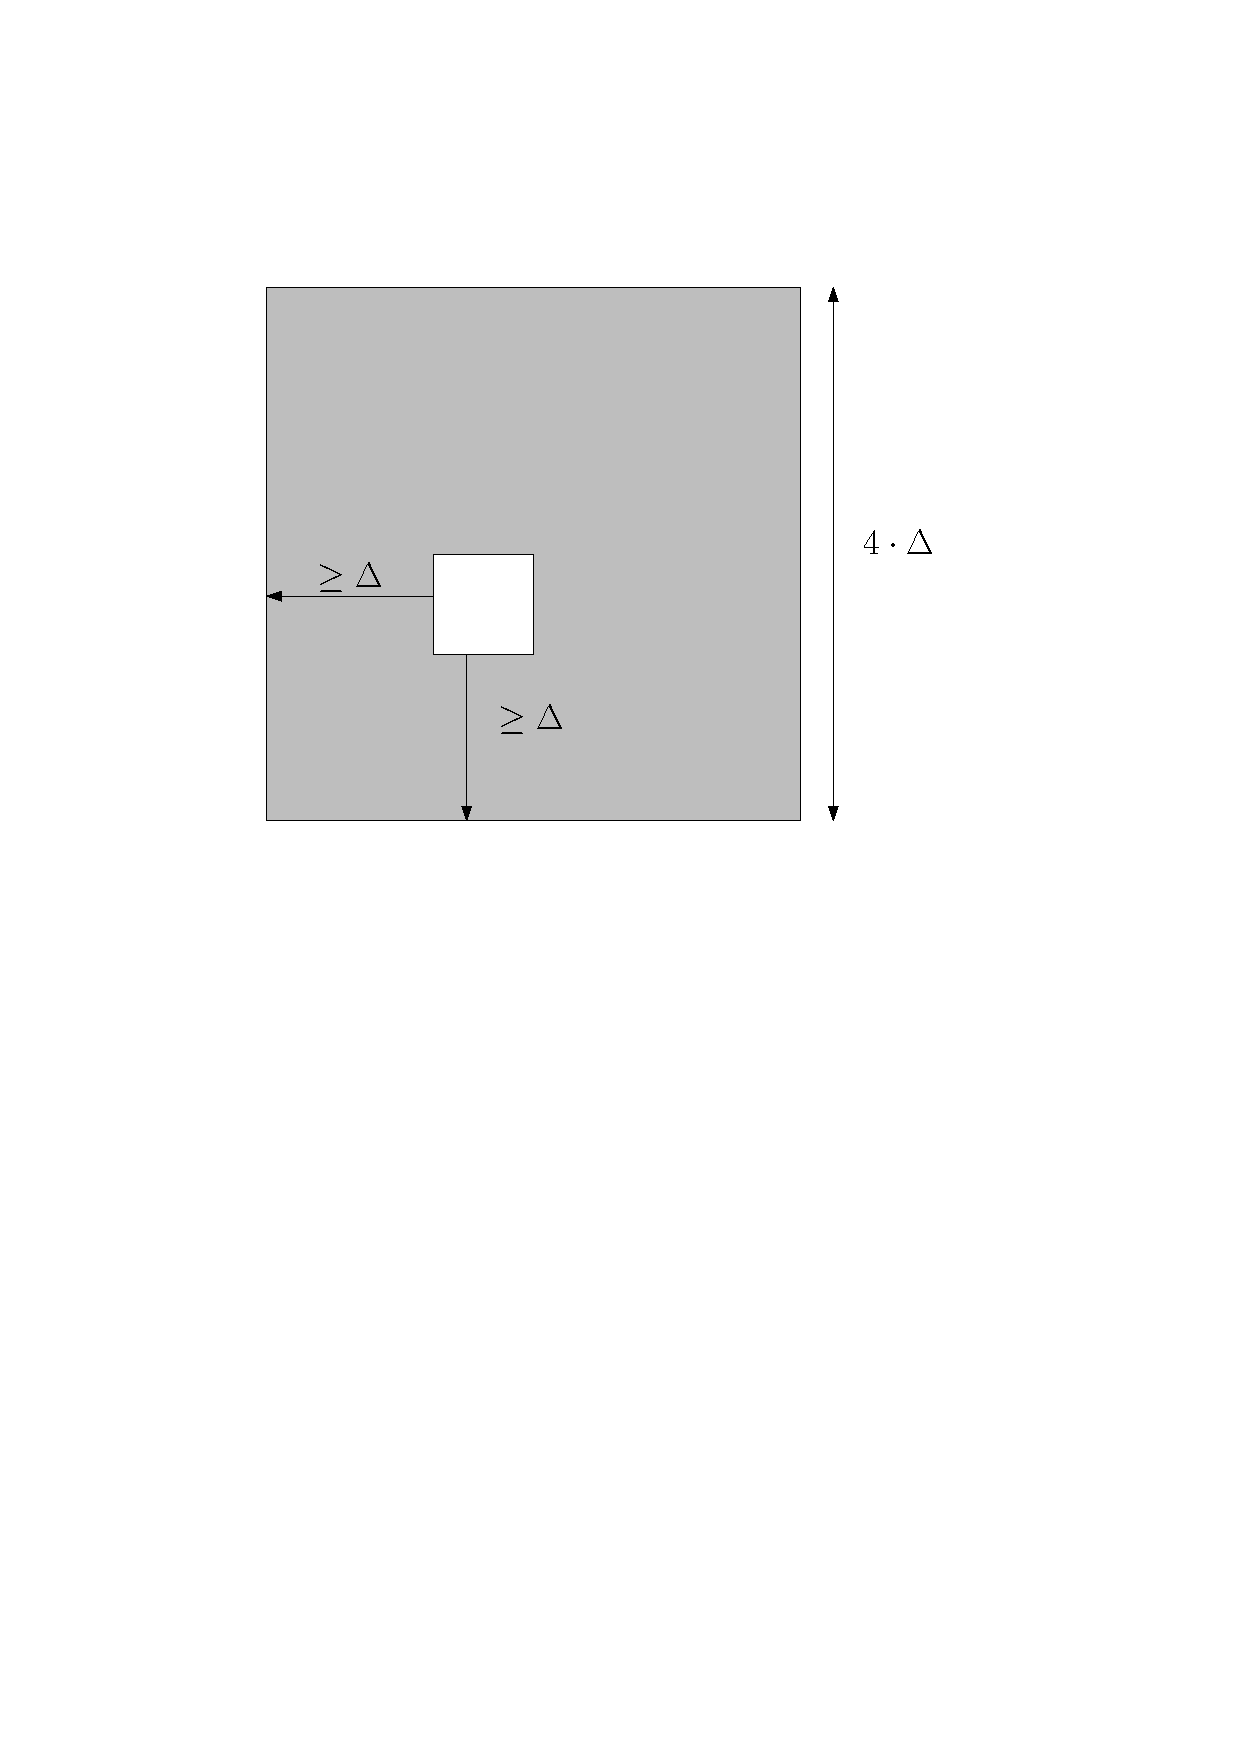
\includegraphics[width=0.5\textwidth]{figures/minimumclearance.pdf}
	\caption{A square-annulus, where the distance from the inner square to the outer 
  			 square, which is $\Delta$, is at least $1/4$ the side length of the outer 
             square which is $4\cdot \Delta$}
	\label{fig:minimumclearancesquareannulus}
\end{figure}

Both the annuli and square faces are subject to the uniform edge property:

\begin{mydef} \textbf{Uniform edge property:} 
\begin{itemize}
	\itemsep0em 
	\item Every edge on the outer square of an annulus has length
		  $1/(4\lceil \alpha \rceil)$ times the side length of the outer square.
	\item Every edge on the inner square has length $1/(4\lceil\alpha\rceil)$ times
		  the side length of the inner square.
	\item The lengths of edges on the boundary of a square cell differ by at
		  most a factor of 4.
\end{itemize}
\end{mydef}

\section{Conforming subdivision theorem}

The conforming subdivision theorem precisely states the properties we expect of our 
subdivision. It is also why this theorem will be proven by construction of the 
conforming subdivision algorithm which we will present in section 
\ref{section:implementationconforming}.

\begin{theorem}
	\label{theorem:conformingsubdivision}
	(Theorem 2.1 in \cite{HershbergerS99}) \textbf{Conforming Subdivision Theorem:} \\
	For any $\alpha\geq 1$, every set of $n$ points in the plane admits a strong
	$\alpha$-conforming subdivision of $O(\alpha n)$ size satisfying the
	following additional properties:
\begin{enumerate}	
	\item All edges of the subdivision are horizontal or vertical,
	\item Each face is either a square of a square-annulus, with subdivided
		boundary,
	\item Each annulus has the minimum clearance property,
	\item Each face has the uniform edge property, and
	\item Every data point is contained in the interior of a square face
\end{enumerate}
	Such a subdivision can be computed in time $O(\alpha n + n\log n)$.
\end{theorem}

This theorem implies that we need to make modifications to the strong conforming 
subdivision of $V$ to accommodate for the edges of the obstacles, because our goal is 
to produce a \textit{conforming subdivision of the free space}. This is done by 
modifying the edges present in the subdivision, s.t. we differentiate between the edges 
introduced by the subdivision construction and the edges of obstacles. We mentioned the 
difference between these before, but for completeness we here present a formal 
definition of these differences.

\begin{mydef}\textbf{Transparent and opaque edges:}\\
    Let the edges in a conforming subdivision of the free space, which are introduced by 
    the subdivision be transparent edges. Equally let the edges in a conforming 
    subdivision of the free space, which are introduced by the original obstacles be 
    opaque edges. 
\end{mydef}

The reason, as mentioned before, we the need to differentiate between these, is due to the 
fact that the algorithm allows wavefronts to pass through transparent edges, but are blocked 
by the opaque edges. We also require that the transparent edges are well-covered in the 
conforming subdivision of the free space, even though they don't need to be strongly 
covered. Due to these requirement, we will slightly alter definition 
\ref{def:wellcoveringwithpara} first and third requirement as such:

\begin{enumerate}
\item[W1$_{fs}$.] Let $e$ be a tranparent edge of $\mathcal{S}$. There exists a set of 
cells $\mathcal{C}(e)\subseteq\mathcal{S}$ such that $e$ is contained in the closure 
of the uinion of cells $\mathcal{U}(e)=\{c|c\in\mathcal{C}(e)\}$.
\item[W3${fs}$.] Let $e$ and $f$ be two transparent edges of $s$ such that $f$ lies on 
the boundary of the well-covering region $\mathcal{U}(e)$. Then the shortest path 
distance between $e$ and $f$ is at least $\alpha\cdot\max(|e|,|f|)$. 
\end{enumerate}

It is worth noting that condition $3_{fs}.$ ensures $e$ does not touch any transparent 
boundary edge of $\mathcal{U}(e)$, although it may touch opaque boundary edges.

\section{Construction of the conforming subdivision}

In this section we go through the basic building blocks used for computing the conforming 
subdivision, $i$-boxes and $i$-quads, and some nice properties and behavior of them. We will go 
through the overlap relation, which is used to make set of equivalence classes of $i$-quads. These 
equivalence classes are the main component for the two algorithms which will calculate the conforming 
subdivision. We will also briefly show a lemma for transforming a $1$-conforming subdivision to a 
$\alpha$-conforming subdivision, for a constant $\alpha$. Finally we will discuss the invariants of 
the of the conforming subdivision algorithms, before moving on to discuss the algorithm in the next 
section. 

\subsection{Definitions of $i$-boxes and $i$-quads}

Before going into the algorithm for constructing the conforming subdivision, wee need
preliminary terminology and definitions.

To make things easy for our selfs, we fix a Cartesian coordinate system in the plane we are 
working with. We say for any integer $i$ and $k$, the $i$'th-order grid in the coordinate 
system is the arrangement of all lines $z = k \cdot 2^i$ and $y = k \cdot 2^i$. This makes a 
grid where each cell (face), is a square of size $2^i \times 2 ^i$, whose lower-left corner 
lies at the point $(k \cdot 2^i, l \cdot 2^i)$, for any pair of integers $k$ and $l$. We will 
refer to such a cell as an $i$-box. Any array of size $4 \times 4$ is called an \textit{i-
quad}, see figure \ref{fig:iquad}.

\begin{figure}[H]
	\centering
	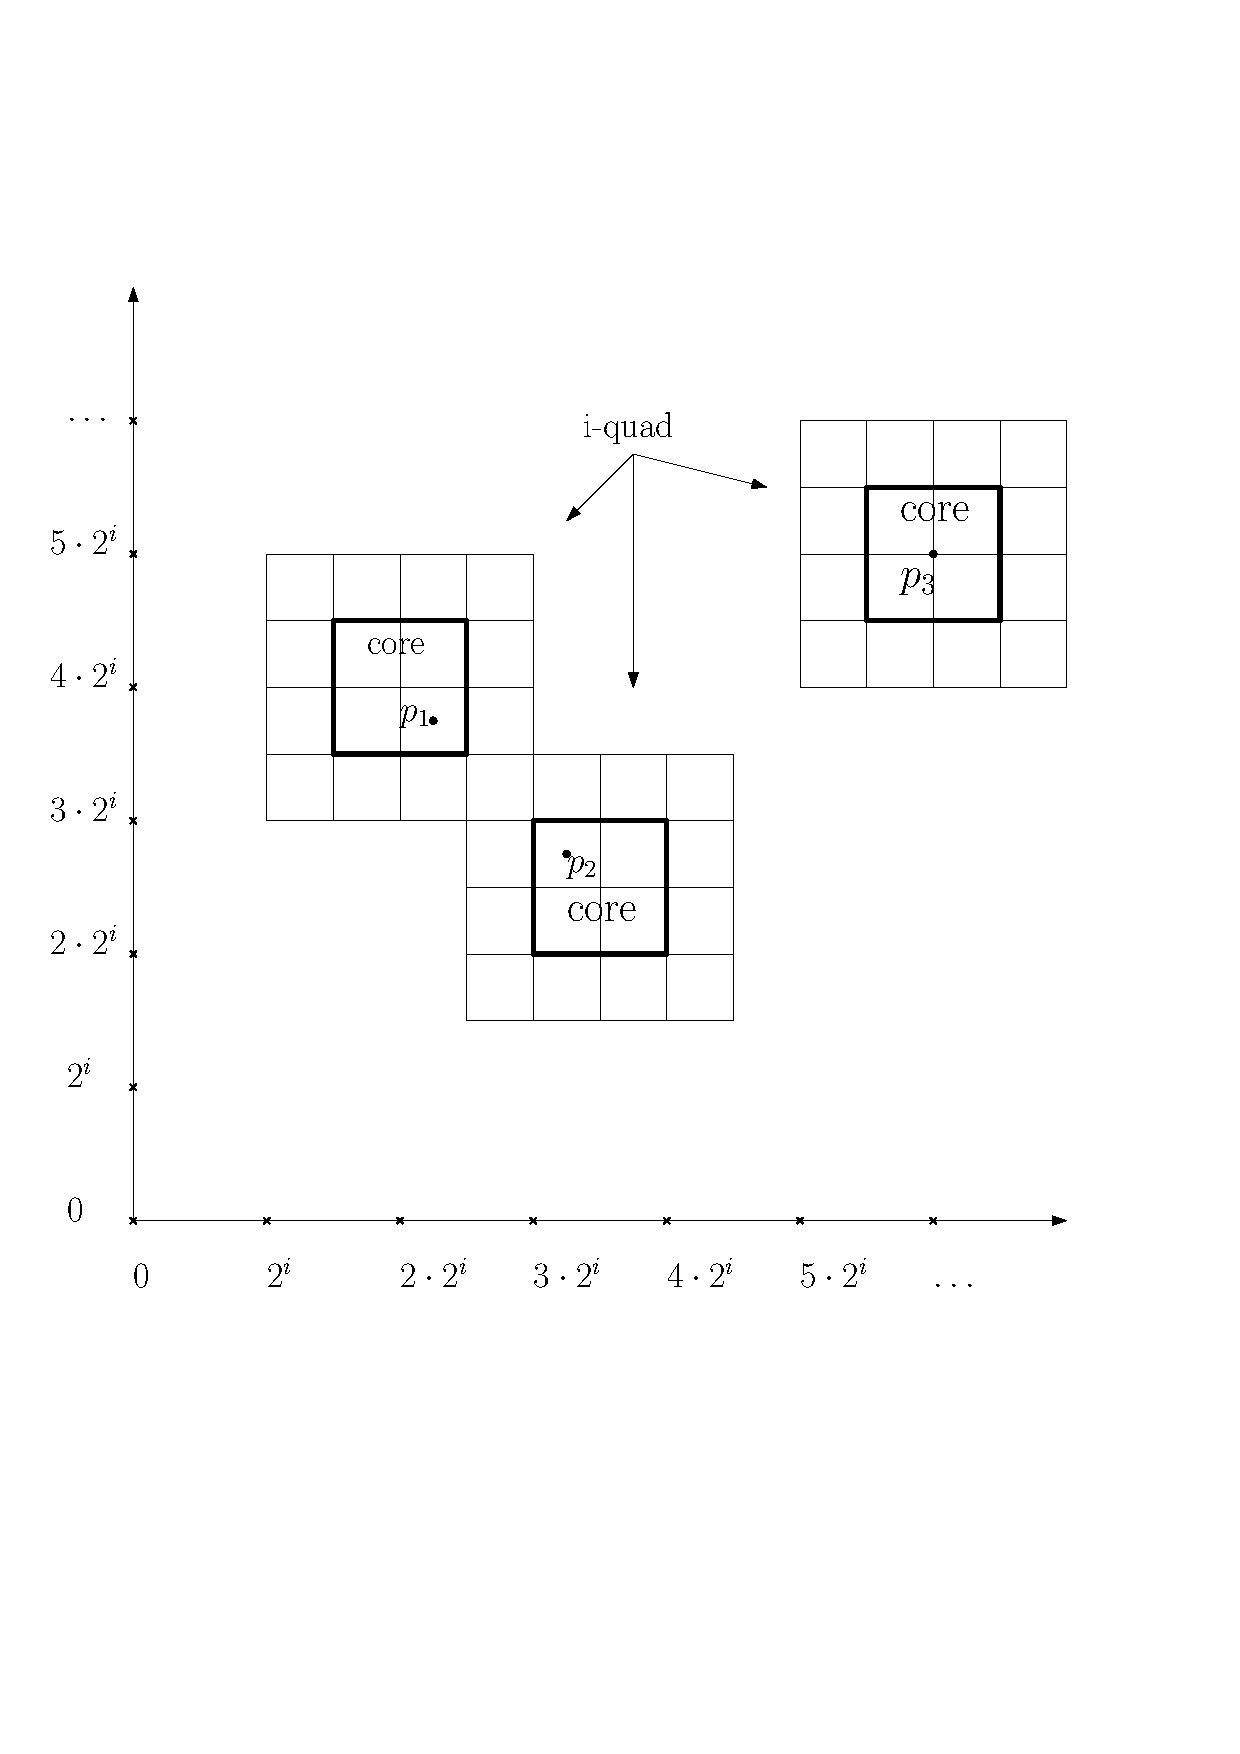
\includegraphics[width=0.7\textwidth]{figures/iquad.pdf}
	\caption{The figure show an example of how i-quads would be grown around the point $p_1, 
    		 p_2$ and $p_3$. Here we also see that in this particular $i$'th stage of growth, 
             that $p_1$ and $p_3$ belong to the same equivalence class, while $p_3$ does 
             not.}
	\label{fig:iquad}
\end{figure}

One could note that, while it is true that the size of an $i$-quad is the same as an 
$(i+2)$-box, an $(i+2)$-box may not be a cell in the $(i+2)$-order grid. So these are not 
always equal. We also refer to the four non-boundary $i$-boxes of an $i$-quad as the core of 
the $i$-quad, see figure \ref{fig:iquad}. By this definition the core is always an $2 \times 
2$ array in the $i$-boxes. One can also observe that an $i$-box $b$ may have up to four 
$i$-quads that contain $b$ in their cores.

The algorithm for building a $1$-conforming subdivision, is in a quad-tree-like fashion where 
we build a partition around the set of points in the plane in a bottomup procedure. This i done 
by \textit{growing} a square box around each data point, until the entire plane is covered by 
these boxes. This is done in a number of discrete \textit{stages} numbered $-2, 0, 2, 4,...$. 
The end goal is to produce a $1$-conforming partition of the points, where the subdivision will 
be a grid with orthogonal cells. Key idea behind the growth process is, each data point $p$ in
stage $i$ is in the core of an $i$-quad. And since we grow the initial box, the data point $p$
will remain in the $i$-quads core, and the following lemma holds inductively, by definition of
the process we have described.

\begin{Lemma}
Each $(i-2)$-quad constructed in stage $(i-2)$ lies in the core of some $i$-quad constructed in 
stage $i$. 
\end{Lemma}

To lower overhead of the algorithm, we only maintain a minimal set of quads at any given $i$-stage.
We denote the set of quads in stage $i$ with $\mathcal{Q}(i)$. This set is partitioned into 
equivalence classes under the transitive closure of an \textit{overlap} relation. 

\begin{mydef} \textbf{(Overlap relation:)} \\
Given any two quads $q$ and $q'$, we say these are in the same equivalence class, by the overlap 
relation, if and only if there is a sequence of quads $q = q_0, q_1, ..., q_m = q' \in 
\mathcal{Q}(i)$, s.t. $q_j$ and $q_{j+1}$ overlap (have common interior point) for all $j = 0, 1, 
..., m - 1$. Further more, let $\{S_1(i), ..., S_k(i)\}$ denote the partition of $\mathcal{Q}(i)$ 
into these equivalence classes in the $i$th stage, and let $\equiv_i$ denote the transitive 
equivalence relation. 
\end{mydef}

We denote a region, or to be more exact the partition of the plane, covered by the quads of one 
class a \textit{component}. By previous definitions we know that a component in stage $i$ either 
is a single $i$-quad, of the a union of $i$-quads where the points in each $i$-quads core, belong 
to the same equivalence class. We differentiate between two types of classes. The first being a 
\textit{simple} component. A component at stage $i$ is simple if

\begin{enumerate}
\item Its outer boundary is an $i$-quad and
\item It contains exactly on $(i-2)$-quad of $\mathcal{Q}(i-2)$ in its interior.
\end{enumerate}

The second type is a complex component. A complex component is complex if it is not simple.

\subsection{Merging of $i$-quad} \label{section:mergingiquad}

In this subsection we show some distance properties that is satisfied by points of the same 
equivalence class at stage $i$, which will be useful in the final algorithm. We say that a quad 
$q$ is a \textit{containing $i$-quad} of a point $u \in V$ if $q \in \mathcal{Q}(i)$ and $u$ lies 
in $q$'s core. We also say that a point $u$ \textit{belongs} to an equivalence class $S \in 
\mathcal{Q}(i)$ if there is a containing $i$-quad of $u$ in $S$.

\begin{Lemma} (Lemma 6.6 in \cite{HershbergerS99}) \label{lemma:6.6HershbergerS99}\\
Let $u$ be a point of $V$ and let $q \in \mathcal{Q}(i)$ be a containing $i$-quad of $u$. Then 
the minimum distance between $u$ and the outer boundary of $q$ is $2^i$.
\end{Lemma}

\begin{proof}
The key idea is the property that $u$ lies in the core of $q$, which we know the size of. Since 
$q$ has side length $2^{i+2}$, and $u$ lies at least a quarter of this distance away from the 
outer boundary, the lemma trivially follows.
\end{proof}

As used earlier in the thesis, we use the notation $d(u,v)$ to denote the distance between the 
points $u$ and $v$.

\begin{Lemma} (Lemma 6.7 in \cite{HershbergerS99}) \label{lemma:6.7HershbergerS99} \\
Let $u$ and $v$ be two points of in the plane that belong to two different equivalence classes of 
$\mathcal{Q}(i)$. Then $d(u,v) > 2 \times 2^i$.
\end{Lemma}

\begin{proof}
Let $q_u$ and $q_v$ be two containing $i$-quads for $u$ and $v$, respectively. Since $u$ and $v$ 
lie in different equivalence classes, these $i$-quads cannot intersect. By Lemma 
\ref{lemma:6.6HershbergerS99}, each of the points lies at least a distance $2^i$ away from 
the outer boundaries of their $i$-quads, which immediately gives a lower bound of $d(u,v) > 2 
\times 2^i$, which proofs the lemma.
\end{proof}

\begin{Lemma} (Lemma 6.8 in \cite{HershbergerS99}) \label{lemma:6.8HershbergerS99}\\
Let $u$ and $v$ be two points in the plane and let $q_u$ and $q_v$, respectively, be the two $i$-quads of $\mathcal{Q}(i)$ containing them. If $q_u \cap q_v \neq \emptyset$, then $d(u,v) < 6 
\times 2^i$.
\end{Lemma}

\begin{proof}
By Lemma \ref{lemma:6.6HershbergerS99}, the maximum distance between $u$ and the outer boundary 
of $q_u$ is at most $3 \times 2^i$. The same holds for $v$ and $q_v$, which implies the upper 
boundary of $d(u,v) < 6 \times 2^i$. See figure \ref{fig:lessthan6i}.
\end{proof}

\begin{figure}[H]
	\centering
	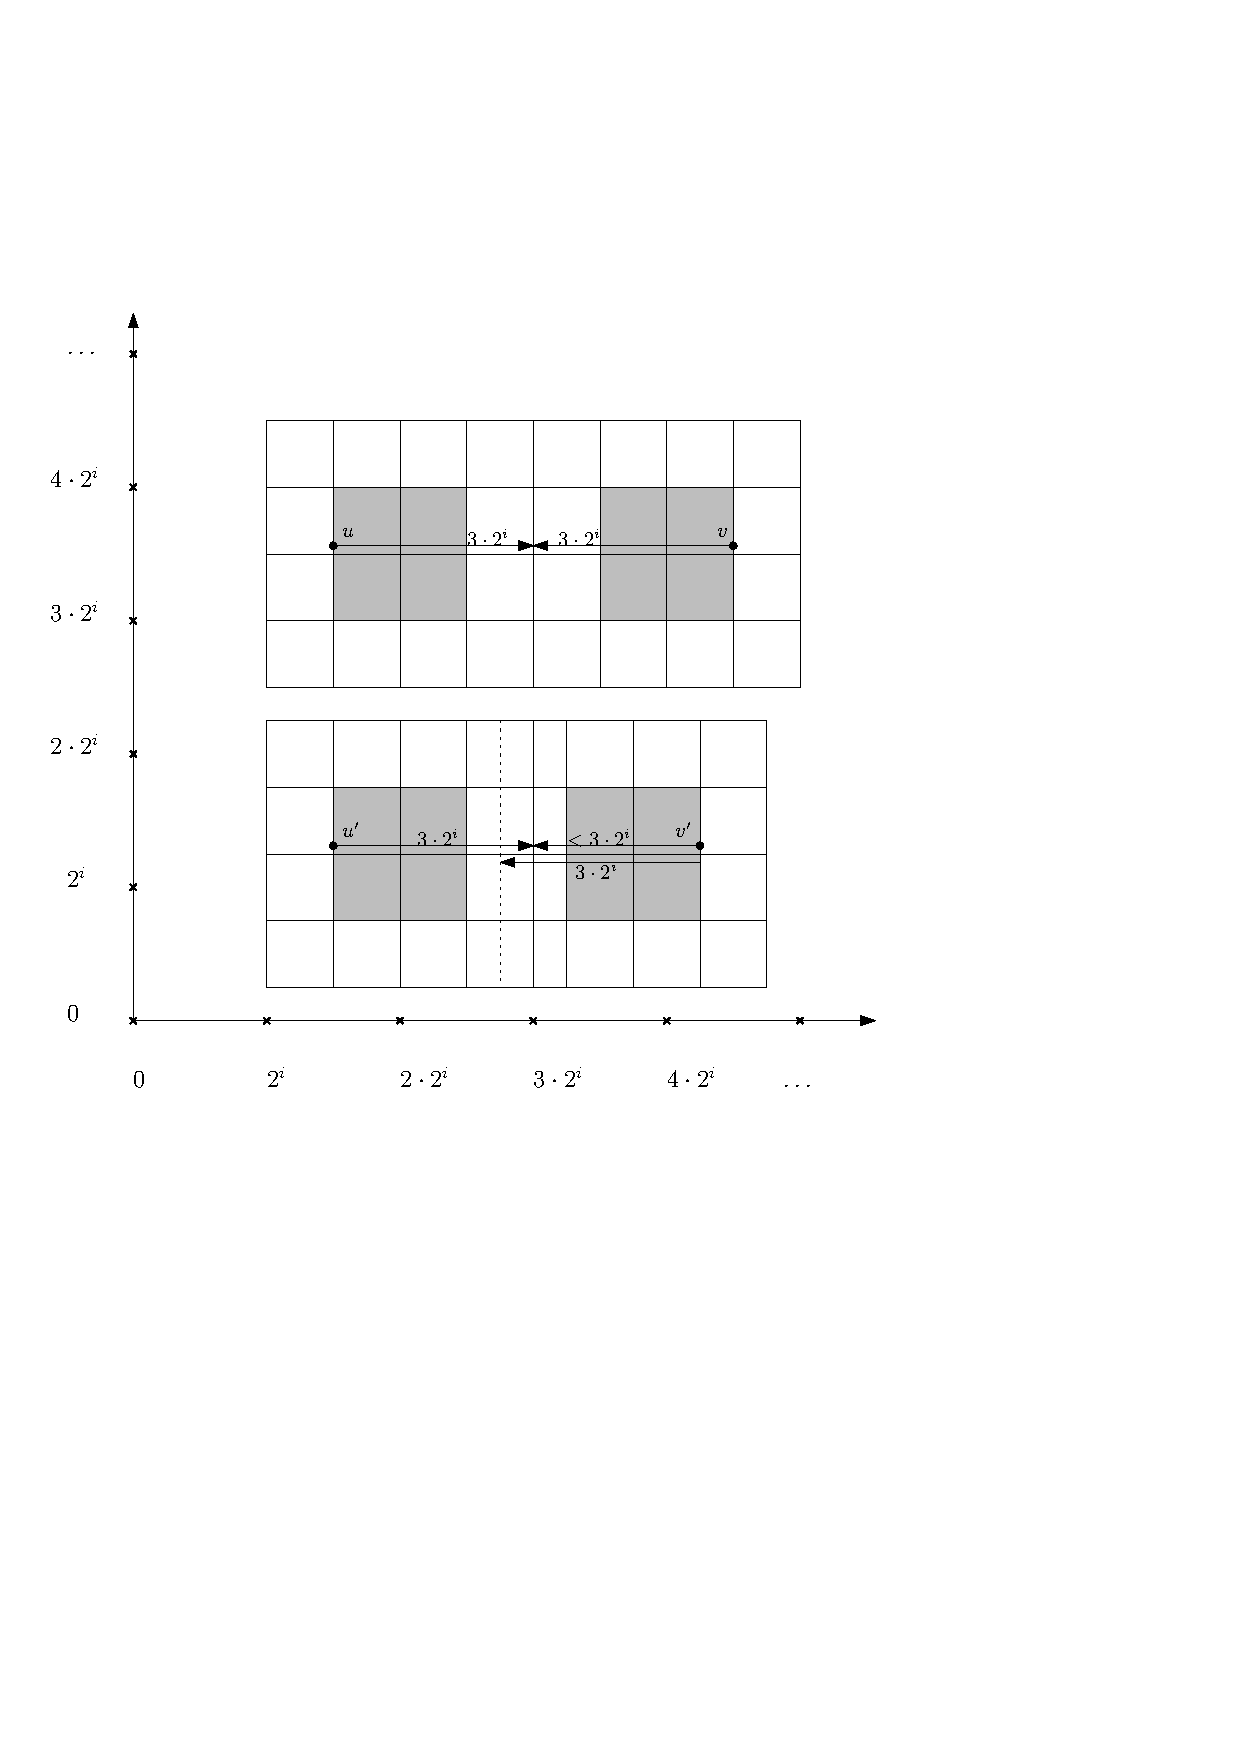
\includegraphics[width=\textwidth]{figures/lessthan6i.pdf}
	\caption{The two top $i$-quads with points $u$ and $v$ are as close as they can be without 
    		 belonging to the same equivalence class, that is not overlapping, and therefore have 
             $d(u,v) = 6 \times 2^i$. The two lower $i$-quads with points $u'$ and $v'$ overlap, and 
             therefore have $d(u,v) < 6 \times 2^i$.}
	\label{fig:lessthan6i}
\end{figure}

\subsection{Transforming $1$-conforming subdivision to $\alpha$-conforming subdivision}

The following lemma shows how to transform a $1$-conforming subdivision into an $\alpha$-conforming 
subdivision of size $O(\alpha\cdot n$ in $O(\alpha\cdot n)$ time. This is quite important for the 
correctness of our algorithm, since we will need the ability to transform the $1$-conforming 
subdivision to an $\alpha$-conforming subdivision.

\begin{Lemma} (Lemma 6.1 from \cite{HershbergerS99}) \label{lemma:6.1HershbergerS99} \\
Let $V$ be a set of $n$ points, and let $\mathcal{S}_1$ be a $1$-conforming 
subdivision for $V$ of size $O(n)$. For any $\alpha>1$, we can build an $\alpha$-conforming 
subdivision $\mathcal{S}_\alpha$ for $V$ with complexity
\end{Lemma}

\begin{proof} Subdivide each edge of $\mathcal{S}_1$ into $\lceil \alpha
	\rceil$ equal-length pieces. Define the well-covering region of each edge
	$e$ in $\mathcal{S}_\alpha$ to be the same as the well-covering region in
	$\mathcal{S}_1$ of which $e$ is a fragment. These operations can performed
	in $O(\alpha\cdot n)$ time. 

We show below that the subdivision thus defined satisfies properties from
	definition \ref{def:aconformingsubdivision}. 

\begin{enumerate}
    \item $\mathcal{S}_\alpha$ has the same set of cells as $\mathcal{S}_1$, so each cell of 
    	  $\mathcal{S}_\alpha$ contains at most one point of $V$ in its closure.
    \item Each internal edge $e_\alpha$ of $\mathcal{S}_\alpha$ is well-covered with 
    	  parameter $\alpha$, since it satisfies the conditions stated in 
          \ref{def:wellcoveringwithpara}. Let $e_1$ be the edge of $\mathcal{S}_1$ of which 
          $e_\alpha$ is a fragment. Let $C_\alpha(e_\alpha)$ be the set of cells of 
          $\mathcal{S}_\alpha$ whose union $\mathcal{U}_\alpha(e_\alpha)$ is the well-
          covering region of $e_\alpha$. Define $\mathcal{C}_1(e_1)$ and $\mathcal{U}(e_1)$ 
          analogously.
    \begin{enumerate}
    	\item $\mathcal{U}_\alpha(e_\alpha)$ covers the same area as $\mathcal{U}_1(e_1)$, 
        	  so $e_\alpha$ is contained in its interior.
        \item Each edge of each cell in $\mathcal{C}_1(e_1)$ is divided in $\lceil \alpha 
        	  \rceil$ pieces in $\mathcal{C}_\alpha(e_\alpha)$ is $O(\alpha)$.
        \item Let $f_\alpha$ be an edge of $\mathcal{S}_\alpha$ on (or outside in the case 
        	  of strongly 1-conforming) the boundary of $\mathcal{U}_\alpha(e_\alpha)$, and 
              let $f_1$ be the edge of $\mathcal{S}_1$ from which it is derived. The 
              Euclidean distance between $e_\alpha$ and $f_\alpha$ is at least as large as 
              the distance between $e_1$ and $f_1$, which is at least $\max(|e_1|,|f_1|)\geq 
              \max(\alpha\cdot|e_\alpha|, \alpha\cdot|f_\alpha|)$.
    \end{enumerate}
    \item Well-covering regions in $\mathcal{S}_\alpha$ are the same as in $\mathcal{S}_1$, 
    	  so each contains at most one vertex of $V$.
\end{enumerate}
Which establishes the lemma.
\end{proof}

\subsection{The invariants}

The main objective of the algorithm is to draw the boundaries of certain components, which in 
the end will give the correct subdivision. Each of these edges will be straight line segments,
all parallel to one the axes, and will be subdividing the plane into orthogonal cells. The 
critical property of our subdivision is the following \textit{conforming property:}

\paragraph{Invariant 1:} For any edge $e$ and cell $c$ of the subdivision, $c$ has an interior 
point within distance $|e|$ of $e$ if and only if $c$ and $e$ are incident (their closures 
intersect). Thus There are at most six cells within distance $|e|$ of any edge $e$. \\

The algorithm will only draw edges of increasing lengths, and so we never need to subdivide 
previously drawn edges inside a component. In order to maintain Invariant 1, the algorithm 
will also enforce the following auxiliary invariant:

\paragraph{Invariant 2:} The boundary of each complex component in stage $i$ is subdivided 
into edges of length $2^i$ that are aligned with the $i$th-order grid\footnote{both invariants 
are as defined in \cite{HershbergerS99} section 6.2}. \\

Through the algorithm the outer boundary of simple components, wont be drawn until just before 
they merge with other components to form complex components. This will show itself very valuable,
since this helps to ensure the upper bound of the size for the final subdivision of $O(n)$.

The algorithm consists of two main sub-algorithms. The first procedure \textit{\textbf{growth}}, 
will take care of simulating the growth of the $(i-2)$-quads to $i$-quads at a stage $i$. The 
second procedure \textit{\textbf{build-subdivision}}, will compute and maintain the equivalence 
classes, and will also draw the subdivision edges (which will satisfy invariant 1 and 2). 

First we will present \textbf{build-subdivision}, and then move on to presenting \textbf{growth}. 
All we need to know about \textbf{growth} for now is, given an $i$-quad $q$, the procedure 
$\mathbf{growth}(q)$ will produce a $(i+2)$-quad containing $q$ inside its core. For a family 
$S$ of $i$-quads, $\mathbf{growth}(S)$ is a minimal set of $(i+2)$-quads satisfying the following:

$$\forall q \in S, \quad \exists \bar{q} \in \mathbf{growth}(S) \quad \text{s.t.} \quad \bar{q} 
= \mathbf{growth}(q)$$

As mentioned earlier, up to four $(i+2)$-quads may contain the $i$-quad $q$ in their cores. So 
to not complicate matter, we will postpone the discussion of how the procedure \textbf{growth} 
chooses $\mathbf{growth}(q)$. For now we will be content with $\mathbf{growth}(q)$ being a 
unique $(i+2)$-quad returned by the procedure \textbf{growth}. We also use the notation $\bar{q}$ 
to denote $\mathbf{growth}(q)$.

\section{Pseudo Code for \textbf{build-subdivision}}

To assure that all components will be simple and disjoint at the initial state, and not complex 
(overlap) we will scale the plane in such a way that either the horizontal or the vertical 
distance between any two points in the plane is at least 1, and no points has a coordinate which 
is a multiple of $1/4$. We compute a $(-2)$-quad for every point $p$ in the plane, with $p$ in 
the upper left corner of the $(-2)$-boxes core. These quads form the initial set of quads in 
$\mathcal{Q}(-2)$. Since no $i$-quad overlaps, they all belong to their own equivalence class, 
and can in this context be regarded as singletons. We proceed to draw the $(-2)$-box around 
each point $p$, which will be contained in the core of the $(-2)$-box, which we won't draw now. 
From this initial setup, one can easily see that the invariants are satisfied, and we are ready 
to proceed with the \textbf{build-subdivision} algorithm:

\begin{algorithm}[H]
	\caption{Algorithm \textbf{build-subdivision}} \label{algorithm:build-subdivision} 
	\begin{algorithmic}[1]
		\While {$|\mathcal{Q}(i)| > 1$} 
        	\State $i = i + 2$
			\State Initialize $\mathcal{Q}(i)=\emptyset$
            \ForEach {equivalence class $S$ of $\mathcal{Q}(i-2)$}
            	\State $\mathcal{Q}(i)=\mathcal{Q}(i)\cup\mathbf{growth}(S)$.
            \EndFor
            \ForEach {pair of $i$-quads $q,q'\in\mathcal{Q}(i-2)$}
            	\If {$q \cap q' \neq \emptyset$}
                	\State Set $q \equiv_i q'$.
                \EndIf
            \EndFor
            \State \multiline{Extend $\equiv_i$ to an equivalence relation by transitive closure, 
            				  and compute the equivalence class}
    		\ForEach {$q\in \mathcal{Q}(i-2)$}
            	\State Let $\bar{q} = \mathbf{growth}(q)$ as computed in step $2-8$
                \If {$q$ is a simple component of $\mathcal{Q}(i-2)$ 
						 but $\bar{q}$ isn't a simple component of
						 $\mathcal{Q}(i)$(*)}
                     \State \multiline{Draw the boundary box of $q$ and subdivide each of its
                     		sides into four edges at the $(i-2)$-order grid lines.}
                \EndIf
            \EndFor
            \ForEach {equivalence class $S$ of $\mathcal{Q}(i)$}
                \State Let $S'=\{q\in\mathcal{Q}(i-2) \quad s.t. \quad 
                	   \mathbf{growth}(s)\in S\}$.
                	\If {$|S|>1$}
                        \State Let $R_1 = \cup_{q\in S'} \{$the core of 
                        	   \textbf{growth}$(q)\}.$
                        \State Let $R_2 = \cup_{q\in S'} \{$the region covered by 
                        	   $q\}.$
                        \State \multiline{Draw $(i-2)$-boxes to fill the region between the 
                        	   boundaries of $R_1$ and $R_2$.}
                        \State \multiline{Draw $i$-boxes to fill the region between the 
                        	   boundaries of $R_1$ and $S$; break each cell boundary 
                               with an endpoint incident to $R_1$ into four edges of 
                               length $2^{i-2}$, to satisfy Invariant 1.}
                    \EndIf
            \EndFor
		\EndWhile
	\end{algorithmic} 
\end{algorithm}
(*)\peter{HOW TO FIX!?}
As we explained earlier, the algorithm runs in discrete stages of $-2, 0, 2, 4, ... $, which we 
see in the increment step of step 2. Step 3 to step 8 computes the $\mathcal{Q}(i)$ from 
$\mathcal{Q}(i-2)$. This is done by growing the previous squares from $\mathcal{Q}(i-2)$, one 
equivalence class at a time, and the see if any of the newly grown squares overlap. If this is 
the case, the belong to the same equivalence class, and should be marked as suck in 
$\mathcal{Q}(i)$. Next in step 10 to 13 we process the simple components of $\equiv_{i-2}$ that 
are about the merge with other components. This is done by checking if the square $q$ which was 
simple before the growth process still would be simple after the growth. If not we draw the 
boundary box of $q$ before the growth, and subdivide its sides into edges of equal length, each 
a quarter of the total side length. The last steps 14 to 20 are dedicated to processing the 
complex components. Here we compute a $S'$ which consists of the $q \in \mathcal{Q}(i-2)$ which 
will grow into the equivalence class $S$ in $\mathcal{Q}(i)$. We will only process if $|S'| > 1$ 
which means $S$ would be complex. Here create two set $R_1$ being the cores of the $i$-quads in 
the complex equivalence class $S$ and $R_2$ being the region covered by the $q$ in $S'$. Should 
these not overlap we fill the region between $R_1$'s and $R_2$'s boundaries with $(i-2)$-boxes. 
In the last step we basically draw the outer boundaries of the $growth(q)$ square, to fill the 
space between the cores, $R_1$, and the outer boundary of $S$, with edges that satisfy our 
invariant. 

This is the overall idea behind the \textbf{build-subdivision} algorithm. This pseudo code, 
while not being efficient enough, gives a good understanding of what we want it to do. We will 
visit this algorithm again in section \ref{section:implementationconforming}, at improve it to 
an $O(n \log n)$ implementation, the needed supporting data structures and more.

\section{Pseudo Code for \textbf{growth}}

The overall idea behind the algorithm for \textbf{growth($S$)} is to build a graph on the quads 
in $S$. 

\begin{algorithm}[H]
	\caption{Algorithm $\mathbf{growth}(S)$} 
	\begin{algorithmic}[1]
		\State Set $\mathbf{growth}(S)=\emptyset$
        \ForEach {pair of quads $q_1,q_2\in S$}
        	\If {$q_1 \cup q_2$ can be contained in a $2 \times 2$ array of $(i+2)$-boxes}
                \State Put an edge between $q_1$ and $q_2$.
            \EndIf
        \EndFor
        \State Compute a maximal matching in the graph computed in Step 1
        \ForEach {edge $(q_1, q_2)$ in the maximal matching}
        	\State Choose an $(i+2)$-quad $\bar{q}$ containing $q_1, q_2$ in its core.
            \State Set $\mathbf{growth}(q_1)=\mathbf{growth}(q_2)=\bar{q}$, and add 
            	   $\bar{q}$ to $\mathbf{growth}(S)$.
        \EndFor
        \ForEach {unmatched quad $q\in S$}
        	\State Set $\mathbf{growth}(q)=\bar{q}$, where $\bar{q}$ is an $(i+2)$-quad 
            	   containing $q$ in its core.
            \State Add $\bar{q}$ to $\mathbf{growth}(S)$.
        \EndFor
	\end{algorithmic} 
\end{algorithm}

Initially we set $\mathbf{growth}(S)$ to be empty. Step 2 to step 4 builds a graph whose 
nodes are the $i$-quads of $S$, with the property that their collective area can be contained 
in a grid of $2 \times 2$ $(i+2)$-boxes. If this is the case we connect the two nodes. In step 
5 we compute a maximal matching of the graph.

\begin{mydef} {Maximal matching} \\
Given a graph $G = (V,E)$, we define a matching $M$ in $G$ to be the set of pairwise 
\textit{non-adjacent} edges; that is, no two edges will have a vertex in common. A maximal 
matching is then defined as a matching $M$ of $G$ with the property that if any edge not in 
$M$ is added to $M$, then $M$ will no longer be a matching. By this definition, we see that 
a maximal matching $M$ is a superset of all other matchings of $G$, where further $M$ can't 
be a subset of the other matching of $G$. See figure \ref{fig:imperfectmatching} and 
\ref{fig:perfectmatching} \peter{wikipedia}
\end{mydef}

\begin{figure}[H]
	\centering
	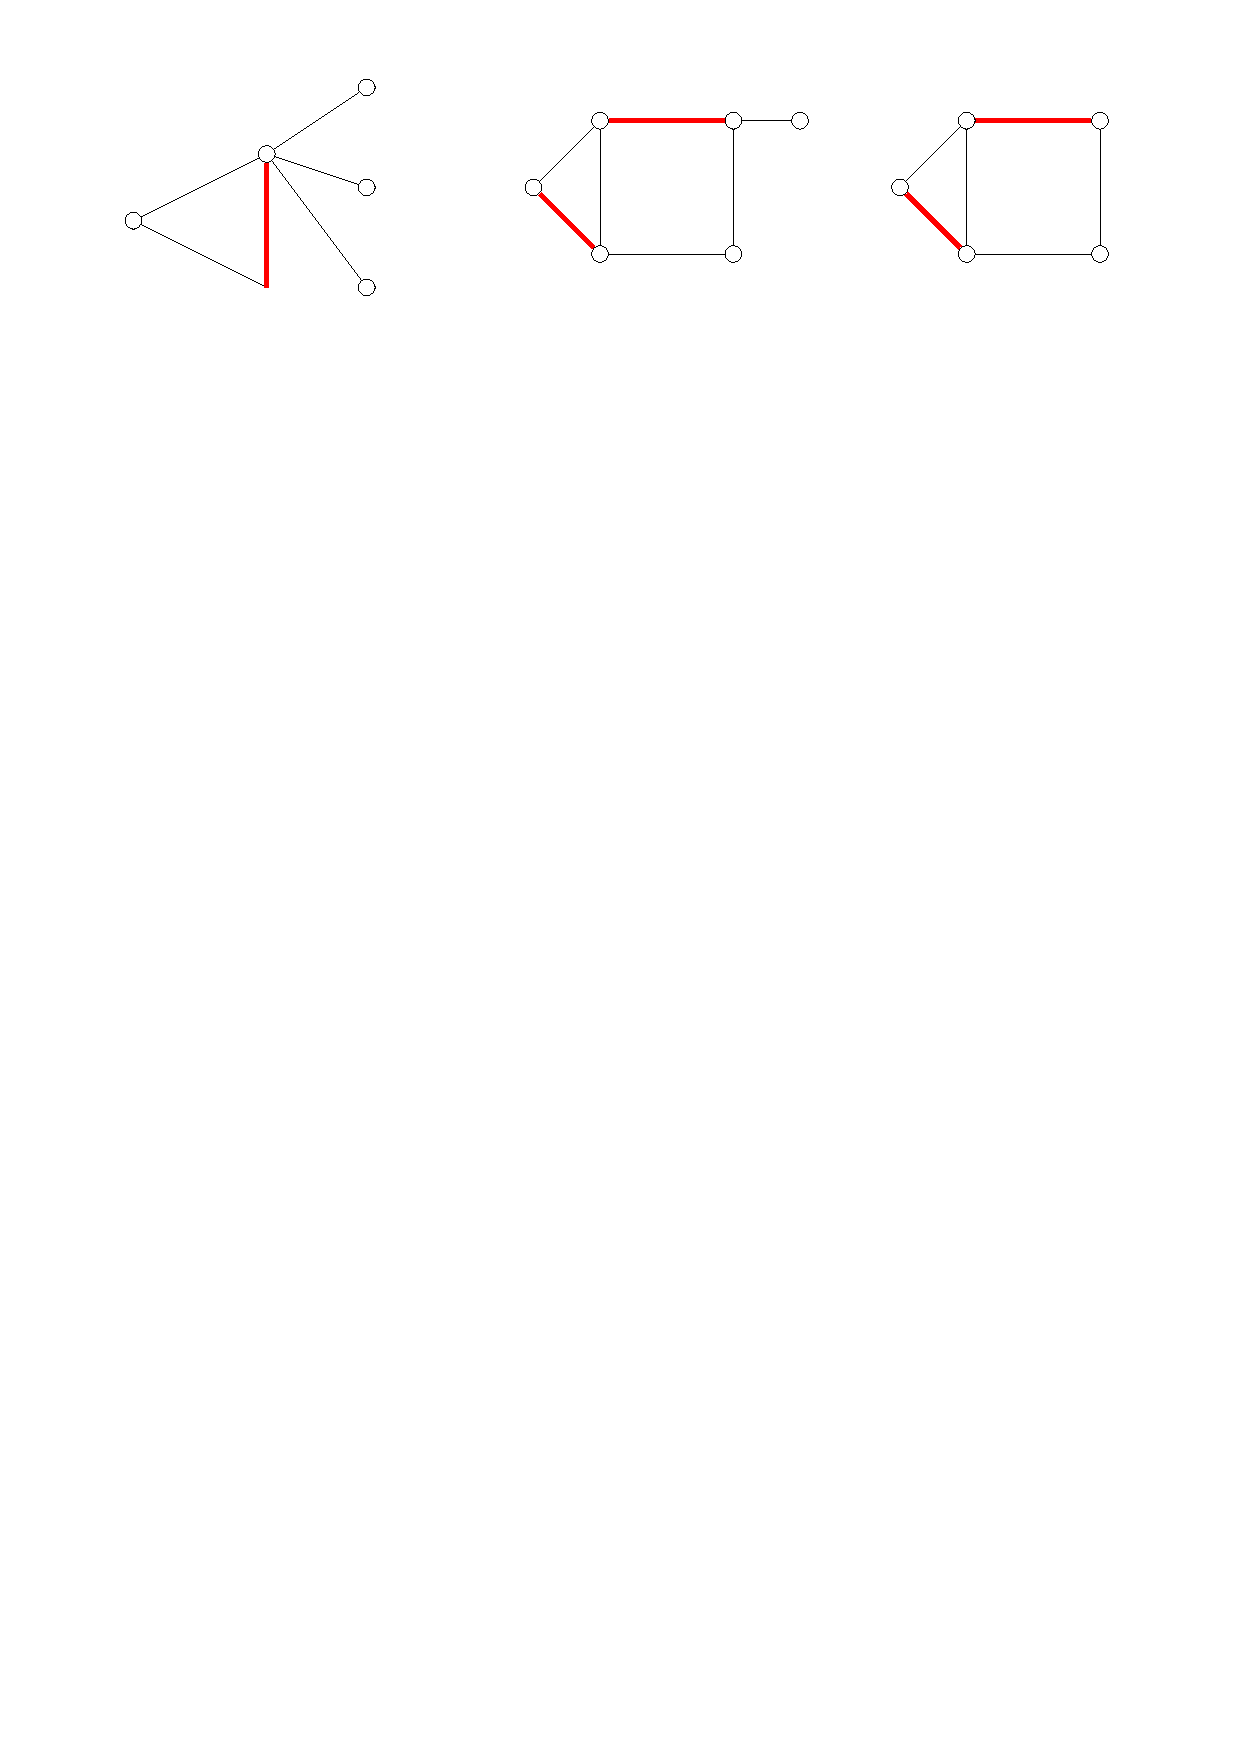
\includegraphics[width=0.7\textwidth]{figures/imperfectmatching.pdf}
	\caption{The figure shows three examples of non maximal matching}
	\label{fig:imperfectmatching}
\end{figure}

\begin{figure}[H]
	\centering
	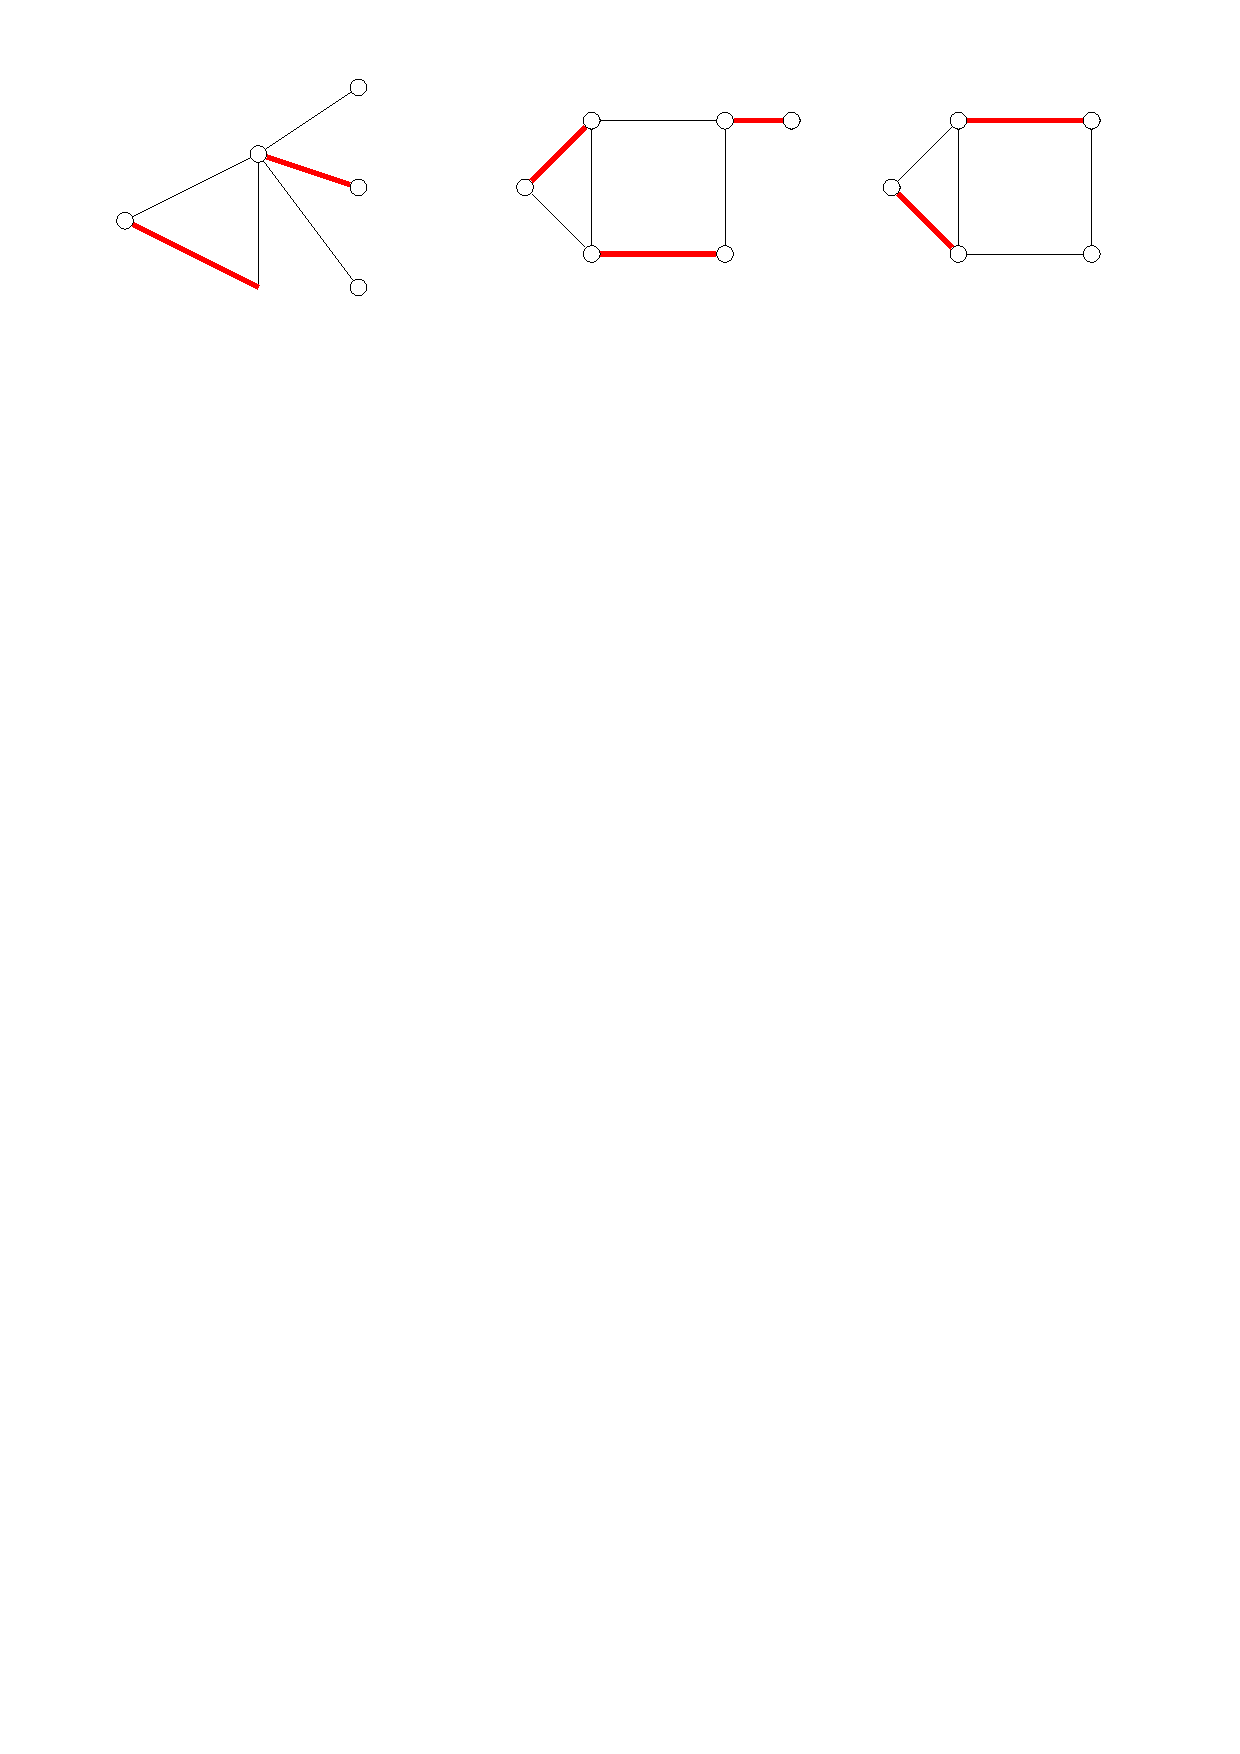
\includegraphics[width=0.7\textwidth]{figures/perfectmatching.pdf}
	\caption{The figure shows three examples of maximal matching, one should notice that the last 
    		 figure have multiple maximum matching, each with two edges.}
	\label{fig:perfectmatching}
\end{figure}

We will save the proof of correctness of the \textbf{growth} algorithm for section 
\ref{section:correctnessgrowth}, but it is worth noting that the maximum node degree of the 
graph build in step 2 to 4, is of constant since, $O(1)$. This is due to the fact that only a 
constant number of $i$-quads can touch any $i$-quad $q$. This implies the maximal matching in 
this graph has $\Theta (|E|)$ edges. Since \textbf{growth} basically maps an $i$-quad to its 
larger counter part in the next stage, each $i$-quad at stage $i$ maps to an $(i+2)$-quad in 
stage $(i+2)$. And since each matching edge, that is the edges marked in step 5, corresponds 
to two $i$-quads that map to the same $(i+2)$-quad, it follows that:

$$|\mathbf{growth}(S)| = |S| - |\Theta(|E|)$$

Later we will show that $|E|$ is a constant fraction of $|S|$ which leads to $|S|$ gradually 
becoming smaller and smaller, which is why the algorithm terminates. We will revisit this fact 
section \ref{section:correctnessgrowth} and give a formal proof, so for now we are content 
with the fact that for each iteration step 5 will compute a maximal matching on gradually 
smaller and smaller graphs.  

Step 5 to 8 constructs a new larger $(i+2)$-quad if two point $q_1$ and $q_2$ would be in it's 
core, and assigns this quad to the equivalence class $S$. The remaining \textit{unmatched} 
quad $q$ are just grown individually and added to the equivalence class $S$.

The fact that any two quads $q, q' \in S$ are contained in the same grown quad $\mathbf{growth}
(q) = \mathbf{growth}(q')$ if their closure intersect is one of the main facts why 
\textbf{growth}$(S)$ runs in time $O(|S| \log |S|)$, which is the overall running time for 
\textbf{growth}.

\section{An $O(n \log n)$ implementation for computing a $1$-conforming subdivision} 
\label{section:implementationconforming}

The following section presents an $O(n \log n)$ implementation of for building a 1-conforming subdivision of the free space. This is done by maintaining the different equivalent classes in $\mathcal{Q}(i)$ for each discrete stage $i$. This is done by making a Delaunay triangulation of the vertices in the plane. When we have this triangulation we can compute the minimum spanning forest by using Kruskal's algorithm, and connect each three if the distance between them is close enough to make the equivalence class merge together. This minimum spanning forest is maintained through each growth stage until all trees in the minimum spanning forest have merged into one tree.

\subsection{Minimum spanning trees}

The minimum spanning tree problem is based on the problem of connecting $n$ points, with $n - 1$ 
edges in such a way that the total weight of these edges remain minimal. More formally, given a 
graph $G = (E,V)$, we can let $w(u,v)$ be a weight function for any two vertices $u$ and $v$ in the 
graph $G$ which returns the weight of the edge between $u$ and $v$ if such an edge exists, and 
$\infty$ if no such edge exists. Then the minimum spanning tree problem is to find a acyclic subset 
$T \subset E$ that connect all vertices, such that the total weight 
$$ w(T) = \sum_{(u,v) \in E} w(u,v)$$
is minimized \cite{IntroToAlg}. The minimum spanning tree would then be the solution to this problem. 

We further say, if the graph $G$ is made up of multiple components then the minimum spanning tree for 
each component, will together form a minimum spanning forest of $G$.

We recall from section \ref{section:mergingiquad} by Lemma \ref{lemma:6.8HershbergerS99}, if two 
$i$-quads $q_u$ and $q_v$ overlap, and therefore at stage $i$ belong to the same equivalence class $S 
\in \mathcal{Q}(i)$ the distance between the two point $u$ and $v$, contained in respectively $q_u$'s 
and $q_v$'s core, has the following  property $d(u,v) < 6 \cdot 2^i$. The $O(n \log n)$ 
implementation of \textbf{build-subdivision} is based upon the fact that, given $V_S$ which is the 
set of points in the core of some equivalence class $S \in \mathcal{Q}(i)$, then the longest edge of 
a minimum spanning tree of $V_S$ has length less than $6 \cdot 2^i$.

Let $V$ be the set of all vertices in the plane we want to build a conforming subdivision around. We 
then define $G(i)$ to be the graph on V which contains exactly those edges whose weight is at most $6 
\cdot 2^i$, and define $MSF(i)$ to be minimum spanning forest of $G(i)$. Here the forest consist of 
each minimum spanning from each component $S \in \mathcal{Q}(i)$.

To show the validity of this idea, we briefly present two Lemma for the correctness of this the above 
assumption. First we show that each point at a stage $i$ only will belong to a single minimum 
spanning tree.

\begin{Lemma} (Lemma 6.9 in \cite{HershbergerS99}) \label{lemma:6.9HershbergerS99}
The points contained in any component $S$ of $\mathcal{Q}(i)$ belong to a single tree of $MSF(i)$.
\end{Lemma}

\begin{proof}
Let $S$ be a random component of $\mathcal{Q}(i)$. By Lemma \ref{lemma:6.8HershbergerS99}, the points 
contained in $S$ can be linked by a tree with edges shorter than $6 \times 2^i$. This implies that 
any bipartition\footnote{bipartition is the grouping of vertices into two groups} of the points of 
$V_S$, has a minimum weight edge linking the two subsets together which is shorter than $6 \times 2^i$. 
The minimum spanning tree of $V_S$ has all edges shorter than $6 \times 2^i$, and therefore $V_S$ 
belongs to a single tree of $MSF(i)$.
\end{proof}

Next we show that if two $i$-quads at stage $i$ don't overlap, then their points will belong to 
different minimum spanning trees in stage $i-2$.

\begin{Lemma} (Lemma 6.10 in \cite{HershbergerS99}) \label{lemma:6.10HershbergerS99}
If $i$-quads $q_1$ and $q_2$ belong to different components of $\mathcal{Q}(i)$, then their points 
belong to different tree of $\mathbf{MSF}(i-2)$.
\end{Lemma}

\begin{proof}
By Lemma \ref{lemma:6.7HershbergerS99} we know that every edge from a point in $q_1$'s core to any point 
outside that core has length greater than $2 \cdot 2^i$. The points of quads $q_1$ and $q_2$ components 
are in the same tree of $MSF(i-2)$ only if every bipartition of $V$ that separates the points of $q_1$ 
from those of $q_2$ is bridged by an edge of length less than $6 \times 2^{i-2}$, this is due to lemma 
\ref{lemma:6.7HershbergerS99}. But the bipartition separating the points of $q_1$'s component of 
$\mathcal{Q}(i)$ from the rest of $V$ has bridge length grater than $2 \times 2^i$, which is due to 
lemma \ref{lemma:6.7HershbergerS99}. Since $2 \times 2^i > 6 \times 2^{i-2}$. the points of $q_1$ and 
$q_2$ must belong to different trees of $\mathbf{MSF}(i-2)$.
\end{proof}

\subsection{\textbf{build-subdivision} implementation}

The final implementation of the \textbf{build-subdivision} procedure is based on an efficient 
construction of the $MSF(i)$ for all $i$ such that $MSF(i) \neq MSF(i-2)$. One way to go 
about this is to compute a Delaunay triangulation of $V$. To understand what a Delaunay triangulation 
is, we start by understanding what a Voronoi digram is. The Voronoi digram is build around points in a 
plane, where the plane partition into a set of cells, where each cell has exactly one point in its 
interior. The special property for each of these cells is that each edge in there border is placed 
between two points, in such a way that the distance from the two points to any point on the edge is the 
same. The Voronoi digram can be computed in $O(n \log n)$ time \cite{CompGeo}. 

Delaunay Triangulation can then be understood as the dual graph of the Voronoi diagram. That is, we can 
build a graph, where the vertex in each cell of the Voronoi diagram gets a edge to another vertex if the 
vertex is a neighboring cell. This gives us a triangulation of the all the points in the plane, where no 
edge overlaps.

The Delaunay triangulation of a plane with points can be done in $O(n \log n)$ time\cite{CompGeo}. and 
then for finding the minimum spanning tree of this triangulation we can run Kruskal's MST 
algorithm\cite{IntroToAlg}. 

Kruskal's algorithm will insert the $O(n)$ edges, made in the Delaunay triangulation, into the, at 
stage $i$, current minimum spanning forest in sorted order from shortest to longest. Any edge that 
might join two trees of the forest is retained, and all other edges are dropped. 

For each edge $e$ added to the forest, we compute $k = 2 \lceil \frac{1}{2} \log_2 (|e|/6) \rceil$, 
which determines the stage $k$ at which $e$ is added to $MSF(k)$\peter{why is this?}. By stopping 
just before each stage change, we produce $MSF(i)$ for each even $i$ such that $MSF(i) \neq MSF(i-2)$ 
in $O(n \log n)$ total time.  

\begin{algorithm}[H]
	\caption{Implementation of \textbf{build-subdivision}}  \label{algo:impl-build-subdivision}
    For each $T \in \mathbf{MSF}(i)$, maintain the corresponding set of $i$-quads in 
    $\mathbf{Q}(i)$ that are the containing quads for the vertices of $T$. Call this 
    set $\mathcal{Q}(i,T)$. \\
    
    Initialize $i=-2$. Initialize $\mathbf{MSF}(-2)$ to be a forest of singleton 
    vertices. For each vertex $v\in V, \mathcal{Q}(-2,\{v\})$ is a singleton quad 
    with $v$ in its core.\\
    
    Maintain a set $\mathcal{N}$ of trees in $\mathbf{MSF}(i)$ such that for each $T 
    \in \mathcal{N}, |\mathcal{Q}(i,T)| > 1$; that is, $T$'s component is not a 
    singleton quad. Initialize $\mathcal{N} = \emptyset$. \\
	\begin{algorithmic}[1]
		\While {$|\mathcal{Q}(i)| > 1$}
        	\State $i_{old} = i$;
            \If {$|\mathcal{N}| > 0$}
            	\State $i = i + 2$
            \Else
            	\State Set $i$ to the smallest even $i' > i$ such that $\mathbf{MSF}
                	   (i') \neq \mathbf{MSF}(i)$
            \EndIf
            \ForEach {edge $e$ of $\mathbf{MSF}(i)$ not in $\mathbf{MSF}(i_{old})$}
            	\State Let $T_1$ and $T_2$ be the trees linked by $e$.
                \ForEach {$T_x \in \{T_1,T_2\}$}
                	\If {$T_x \in \mathcal{N}$}
                    	\State Remote $T_x$ from $\mathcal{N}$.
                    \Else
                    	\State compute the singleton $(i-2)$-quad in $\mathcal{Q} 
                        	   (i-2 ,T_x)$.
                    \EndIf
                \EndFor
                \State Join $T_1$ and $T_2$ to get $T'$, and put $T'$ in 
                	   $\mathcal{N}$.
                \State Set $\mathcal{Q}(i-2,T') = \mathcal{Q}(i-2, T_1) \cup 
                	   \mathcal{Q}(i-2,T_2)$
            \EndFor
            \ForEach {$T\in\mathcal{N}$}
            	\State Initialize $\mathcal{Q}(i,T) = \emptyset$.
                \ForEach {equivalence class $S$ of $\mathcal{Q}(i-2,T)$}
                	\State $\mathcal{Q}(i,T) = \mathcal{Q}(i,T) \cup \mathbf{growth}
                    	   (S)$.
                \EndFor
                \State Compute the equivalence classes of $\mathcal{Q}(i,T)$ by plane
                	   sweep.
                \State perform Steps 10 through 20 of algorithm 
                	   \ref{algorithm:build-subdivision} on $\mathcal{Q}(i,T)$.
                \If {$|\mathcal{Q}(i,T)=1$}
                	\State Delete $T$ from $\mathcal{N}$.
                \EndIf
            \EndFor
        \EndWhile
	\end{algorithmic} 
\end{algorithm}

To give a better overview, we include step 10 through 20 from algorithm 
\ref{algorithm:build-subdivision} below.

\begin{algorithm}[H]
	\caption{step 10 to 20 from Algorithm \ref{algorithm:build-subdivision}}  
	\begin{algorithmic}[1]
        \ForEach {$q\in \mathcal{Q}(i-2)$}
            \State Let $\bar{q} = \mathbf{growth}(q)$
            \If {$q$ is a simple component of $\mathcal{Q}(i-2)$ 
                but $\bar{q}$ isn't a simple component of
                $\mathcal{Q}(i)$(*)}
                \State \multiline{Draw the boundary box of $q$ and subdivide each of its
                sides into four edges at the $(i-2)$-order grid lines.}
            \EndIf
        \EndFor
        \ForEach {equivalence class $S$ of $\mathcal{Q}(i)$}
            \State Let $S'=\{q\in\mathcal{Q}(i-2) \quad s.t. \quad 
            \mathbf{growth}(s)\in S\}$.
            \If {$|S|>1$}
                \State Let $R_1 = \cup_{q\in S'} \{$the core of 
                \textbf{growth}$(q)\}.$
                \State Let $R_2 = \cup_{q\in S'} \{$the region covered by 
                $q\}.$
                \State \multiline{Draw $(i-2)$-boxes to fill the region between the 
                boundaries of $R_1$ and $R_2$.}
                \State \multiline{Draw $i$-boxes to fill the region between the 
                boundaries of $R_1$ and $S$; break each cell boundary 
                with an endpoint incident to $R_1$ into four edges of 
                length $2^{i-2}$, to satisfy Invariant 1.}
            \EndIf
        \EndFor
	\end{algorithmic} 
\end{algorithm}


There are a couple of things worth noticing about algorithm \ref{algo:impl-build-subdivision}. For once 
we only process stages in which something happens, indicated by the choice of $i$ in step 2 to step 6. 
These cases are if $MSF(i)$ changes, that is two trees merge into one, or there are complex components 
of $\mathcal{Q}(i)$ whose \textbf{growth} computation is nontrivial. By this we mean we only compute 
$growth(S)$ for complex components and for simple components that will merge with other components soon, 
and compute the equivalence classes of $\mathcal{Q}(i)$ only for this same set of quads. Simple 
components that are well-separated from others are not involved in these computations since they by 
nature are quite trivial. 

The running time of this algorithm is dominated by the $O(k \log k)$ required for a plane sweep \cite{CompGeo} of $k=|\mathcal{Q}(i,t)|$ quads in step 20. There are $O(k)$ quads in complex components either in $\mathcal{Q}(i,T)$ or in $\mathbf{Q}(i+2,T)$, so there are $O(k)$ edges drawn for these quads at stage $i$ or $i+2$. We amortize this cost by charging $O(\log k)$ per edge of the subdivision getting $O(n\log n)$ time overall. The computation of the Delaunay triangulation and the minimum spanning forest contributes a term of the same asymptotic magnitude.\\
We have established the following lemma.

\begin{Lemma} (Lemma 6.11 in \cite{HershbergerS99}) \label{lemma:6.11HershbergerS99}\\
Algorithm build-subdivision can be implemented to run using $O(n \log n)$ standard operations on a real RAM, plus $O(n)$ floor and $base_2$ logarithm operation.
\end{Lemma}